\section{Thrust distribution}

In order to validate the ALEPH archived data sample and our understanding,
an analysis of the thrust distribution ($T$) is performed with LEP1 archived
data. The distributions are corrected for the detector response by ALEPH MC
produced in 1994. The results are unfolded by a Bayesian unfolding method. The size of the correction factor is small in the mid-$T$
and becomes larger as we go to smaller $T$ or larger $T$ regions.

%\begin{figure}[H]
%\centering
%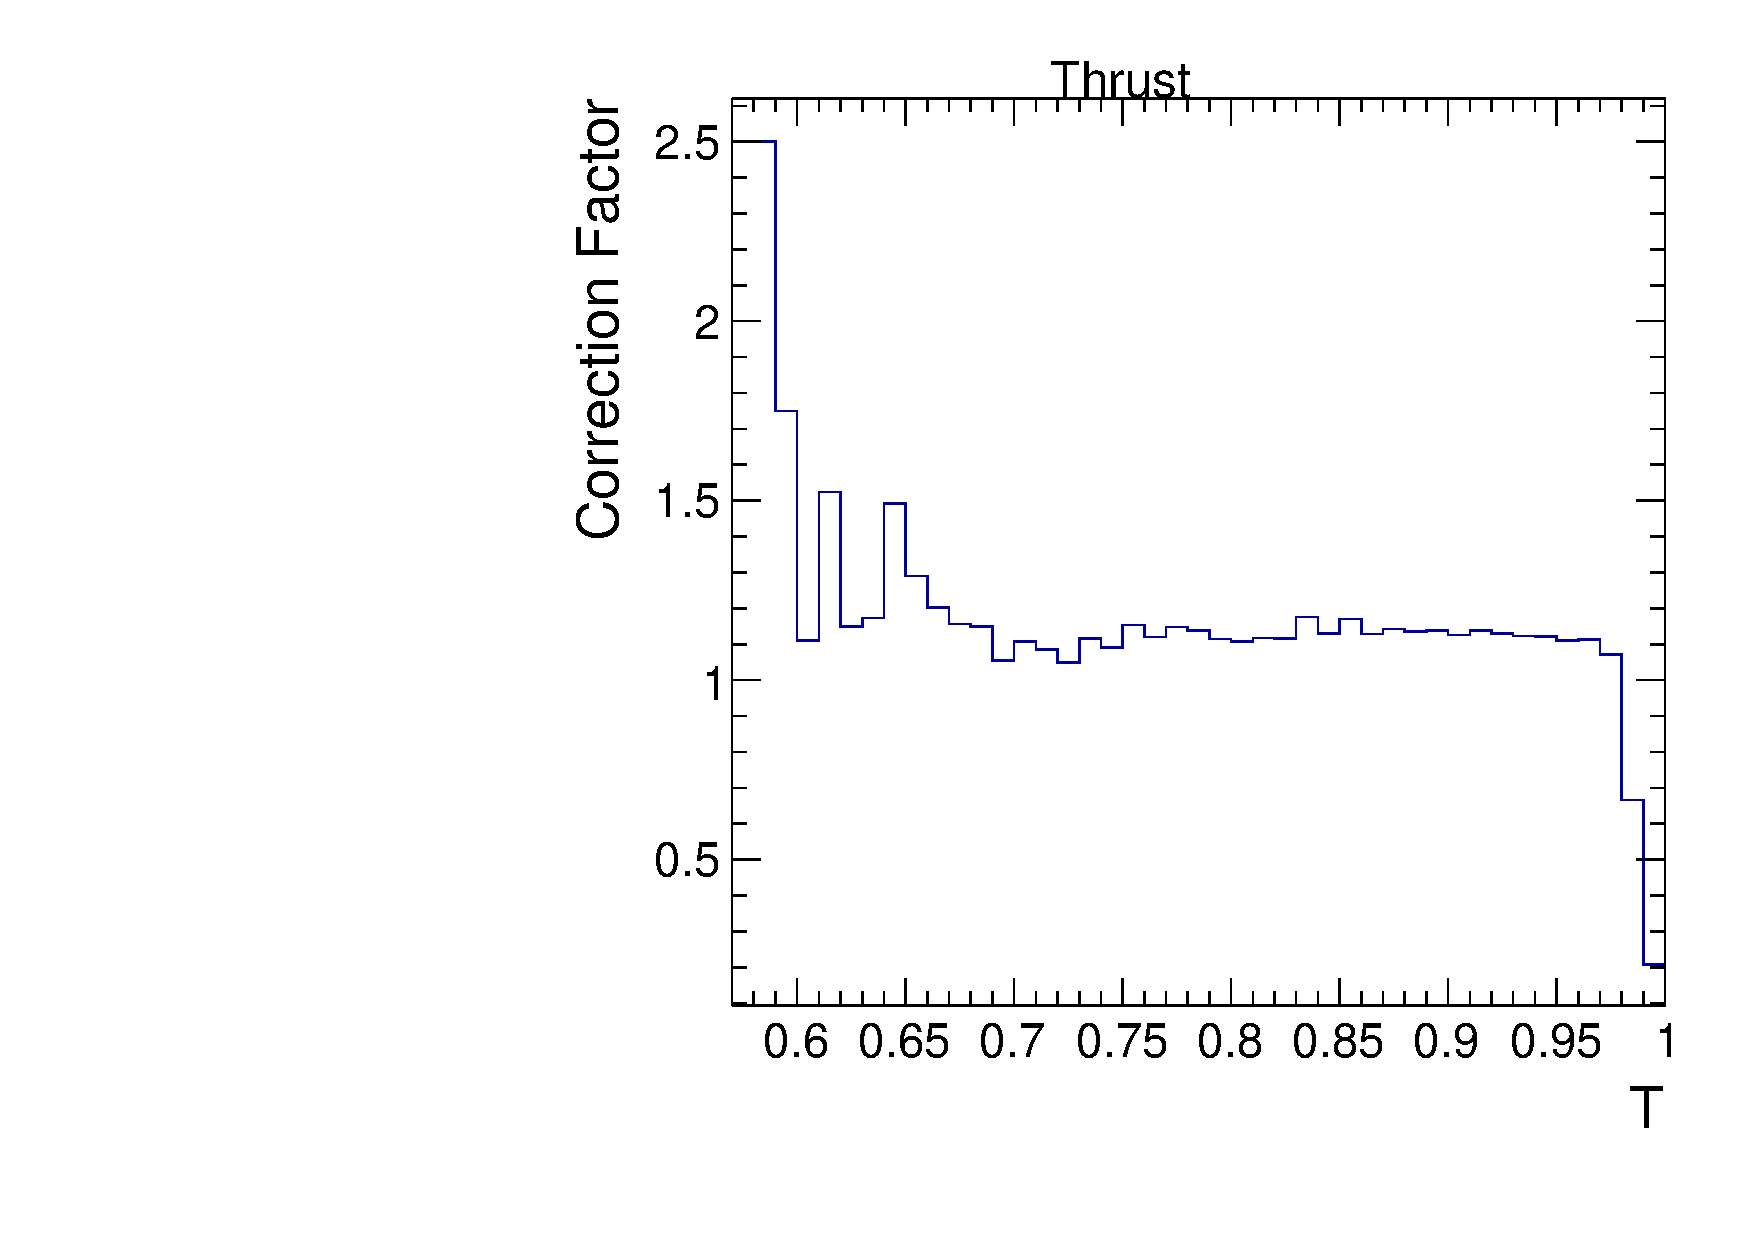
\includegraphics[width=.5\textwidth]{images/Thrust/correction.pdf}
%\caption{The correction factor for the Thrust distribution measurement obtained from ALEPH MC.}
%\label{fig:ThrustCorr}
%\end{figure}

Figure~\ref{fig:ThrustResults} shows the corrected thrust distribution from ALEPH archived data. The results are compared to ALEPH
publications~\cite{Barate:1996fi,heister:2003aj}. As shown in the figure, a very good agreement between ALEPH archived data from this note
and ALEPH publications in the low $T$ region. In the $T\sim 1$ region, a small difference at the level of 0-10\% is observed between this work
and the ALEPH publication in 2004~\cite{heister:2003aj}. This could be due to the difference in unfolding procedure, the dataset used and the event selection criteria.


\begin{figure}[H]
\centering
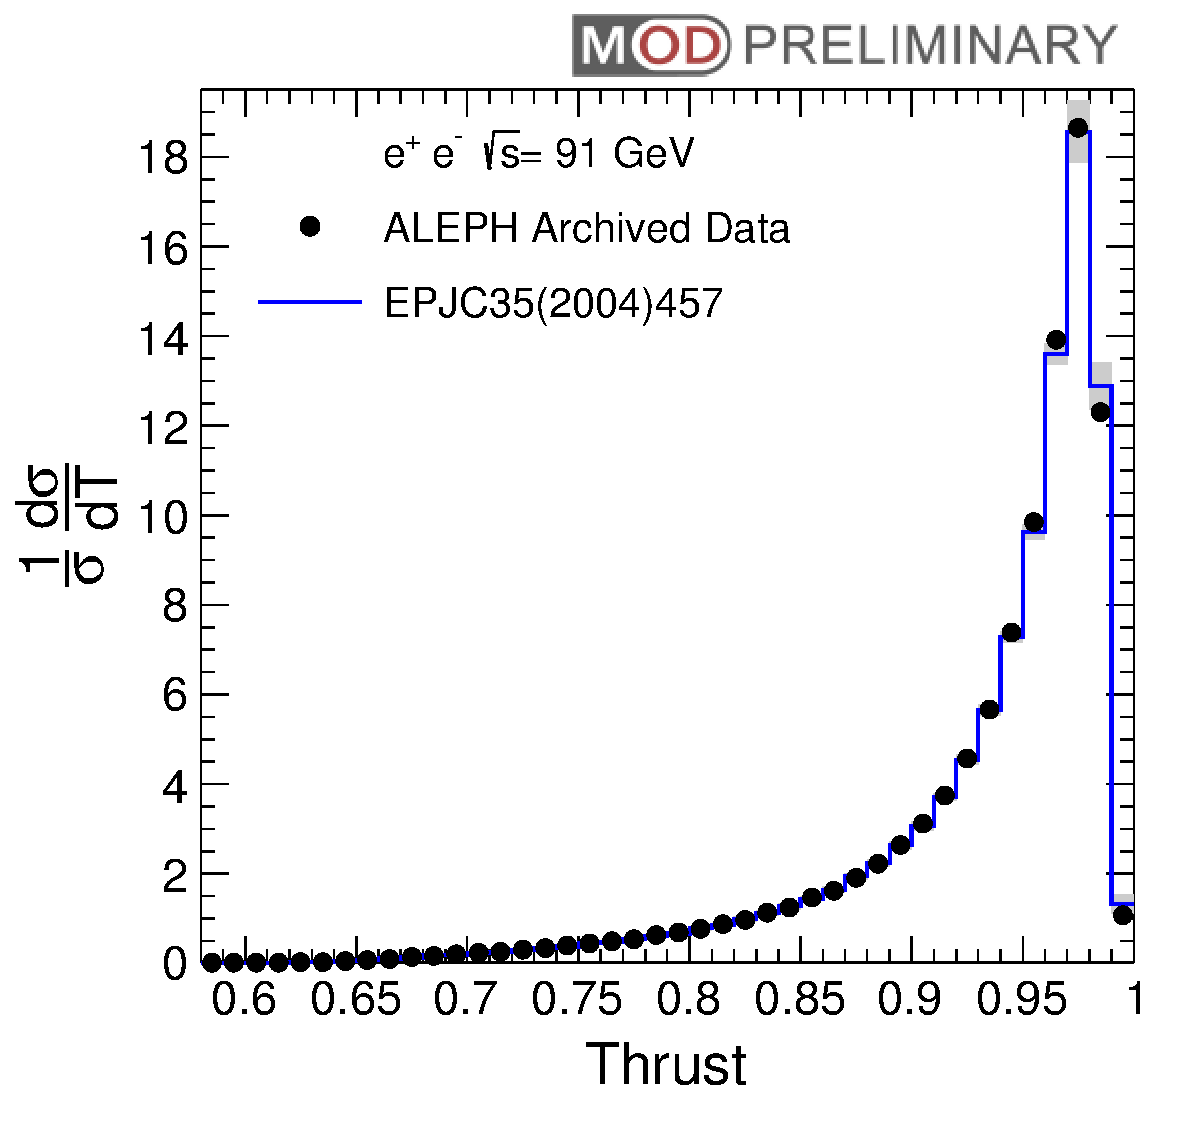
\includegraphics[width=.49\textwidth]{images/Thrust/ThrustResult.pdf}
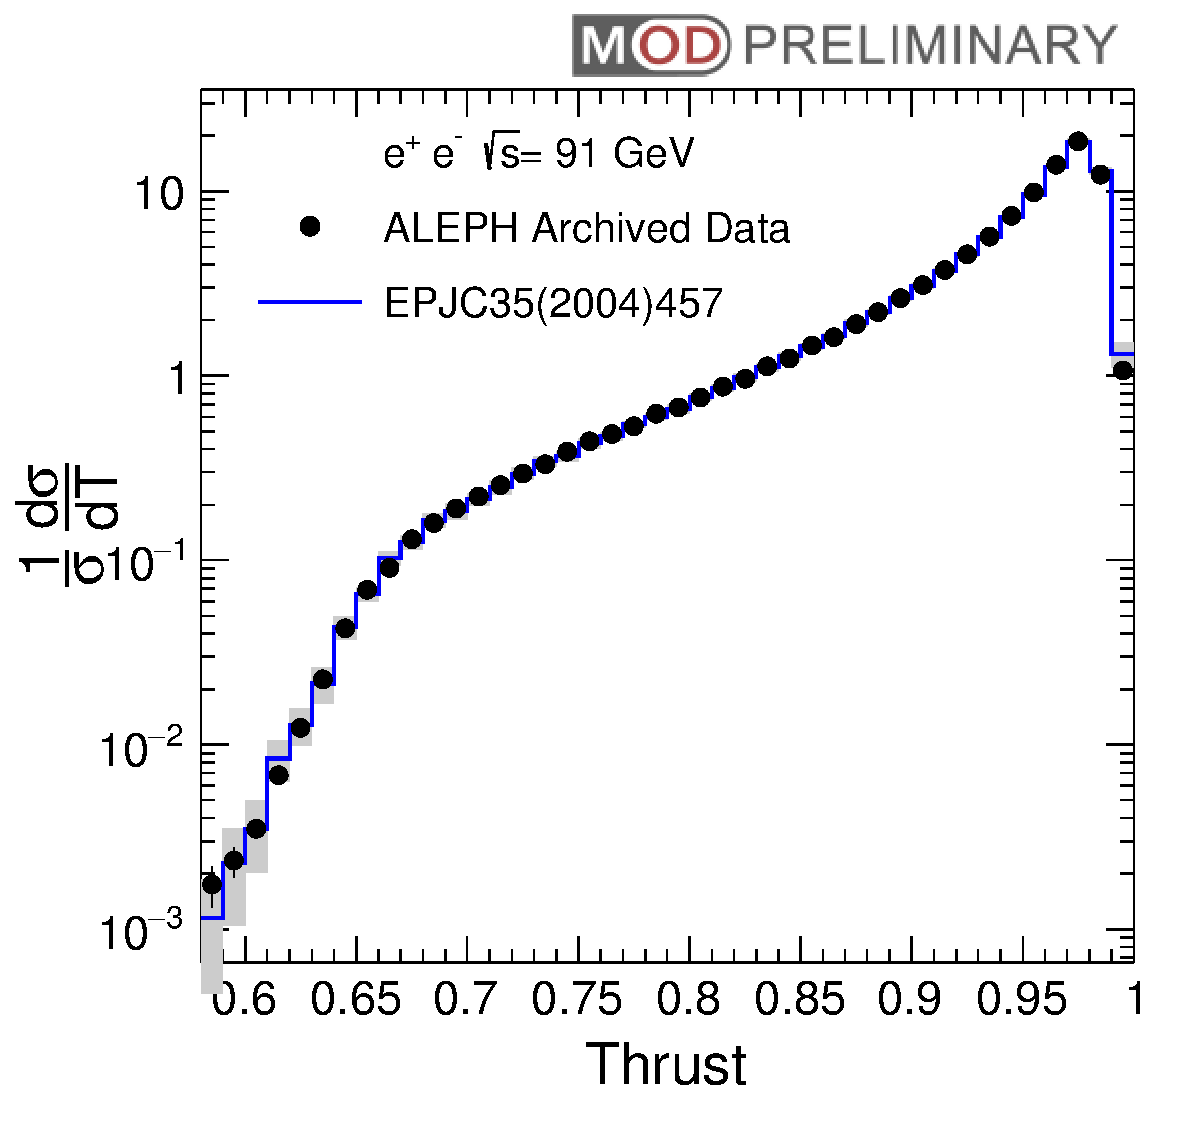
\includegraphics[width=.49\textwidth]{images/Thrust/ThrustResultLogY.pdf}
\caption{The corrected thrust distribution from ALEPH archived data compared to previous publications in linear and log scale.}
\label{fig:ThrustResults}
\end{figure}
